%=============================================
\section{Results}
%=============================================

\begin{figure}
    \centering
    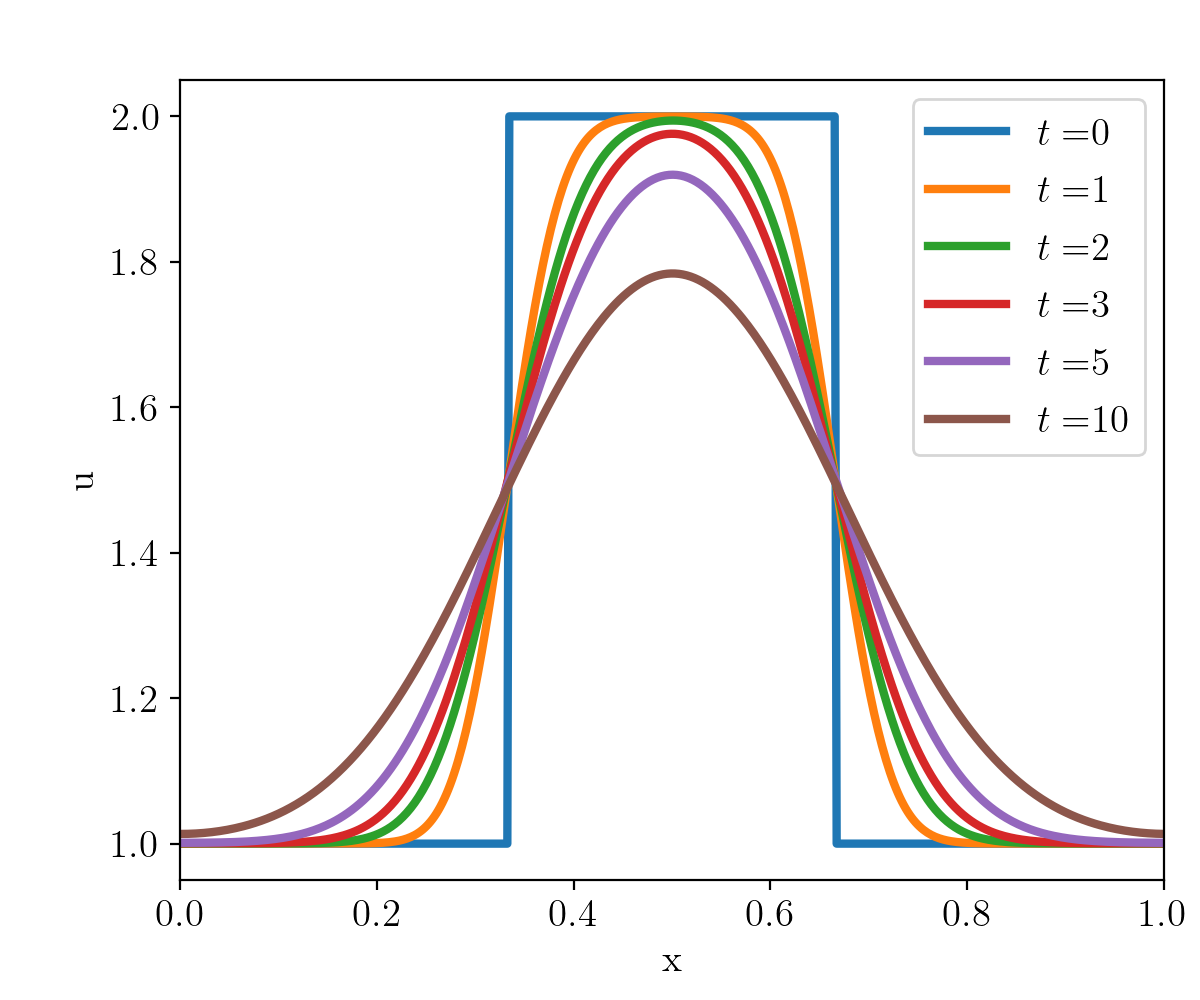
\includegraphics[width=.5\textwidth]{
    ./figures/advection-1D-step.png}%
    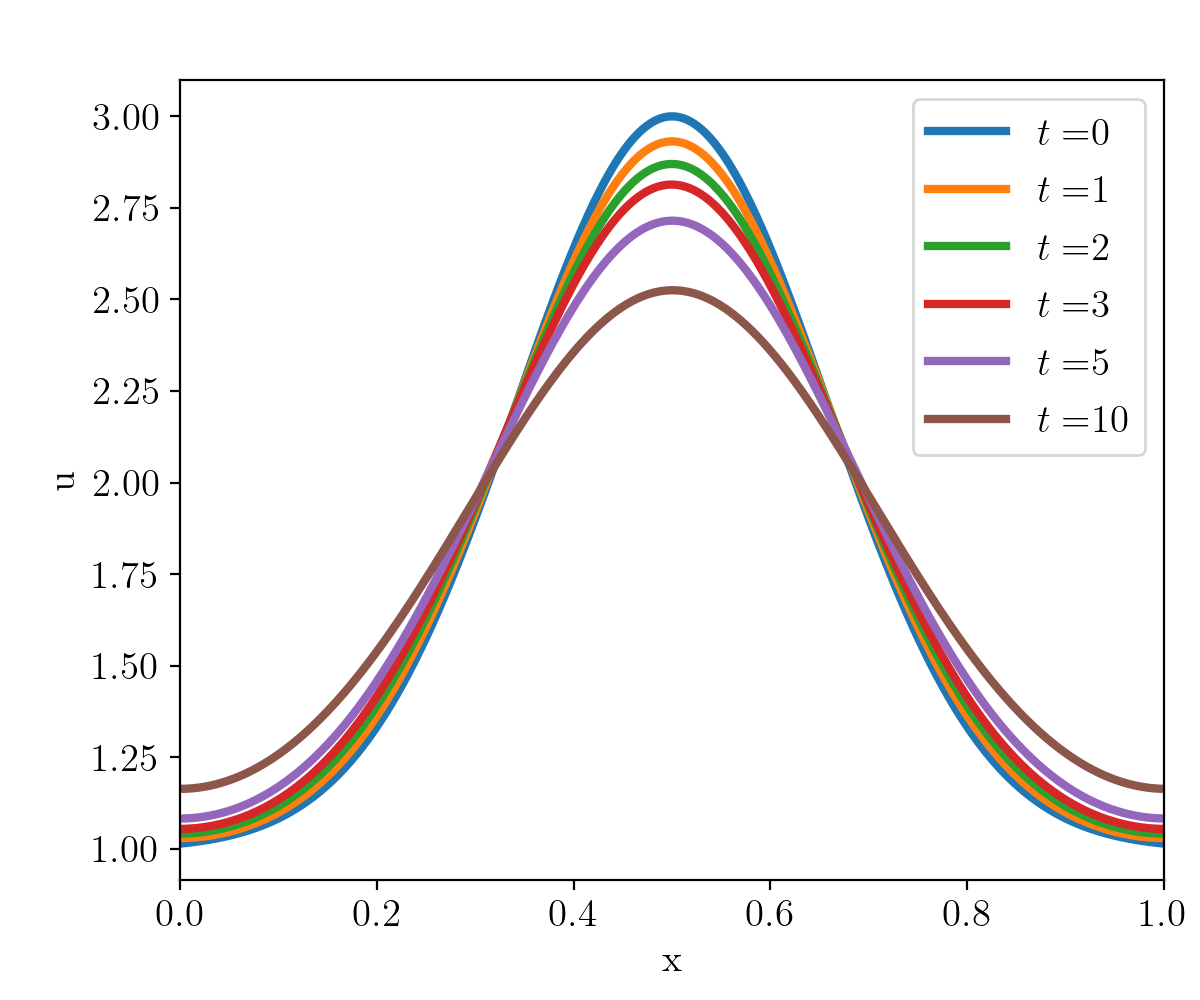
\includegraphics[width=.5\textwidth]{
    ./figures/advection-1D-gaussian.png}%
    \caption{
The solution of the linear advection equation with constant coefficient $a = 1$ (in arbitrary
units). On the left, the initial conditions are a step function, on the right, they are a
Gaussian. The results at $t > 0$ have been repositioned to the original position to demonstrate
how the initial shape changes over time, which according to the analytical solution shouldn't
happen.
    }%
    \label{fig:linear-advection-results}
\end{figure}

Figure~\ref{fig:linear-advection-results} shows the solution using our first 
order finite difference method for a step function and a Gaussian at different 
times, moved back to the original position to demonstrate how the initial shape 
changes over time. According to the known analytical solution, which says that
$q(x, t)$ should only be translated with $a t$ as time evolves, this is wrong.

The reason is an effect called ``numerical diffusion''. It arises due to the nature
of the discrete method, and is unfortunately unavoidable.

The purpose of this Section in the text is to give you a known result you can compare
yours to, and in particular to mention that the effects of numerical diffusion are
natural and expected. You don't need to understand them to successfully debug the solver.
However, for the interested readers, an explanation is given below.

Consider our finite difference approximation of the eqation of linear advection:

\begin{align}
    \frac{q_i^{n+1} - q_i^n}{\Delta t} + a\frac{q^{n}_{i} - q_{i-1}^n}{\Delta x} = 0
    \label{eq:numerical-diffusion-finite-difference}
\end{align}

The terms $q_i^{n+1}$ and $q_{i-1}^n$ can be Taylor-expanded to second order in $\Delta t$ and
$\Delta x$:

\begin{align}
    q_i^{n+1} &=
        q_i^n + \Delta t \DELDT{q} +
        \frac{\Delta t^2}{2} \frac{\del^2 q}{\del t^2} + \mathcal{O}(\Delta t^3)
    \label{eq:taylor-un+1}\\
    q_{i-1}^{n} &=
        q_i^n - \Delta x \DELDX{q} +
        \frac{\Delta x^2}{2} \frac{\del^2 q}{\del x^2} + \mathcal{O}(\Delta x^3)
    \label{eq:taylor-ui-1}
\end{align}


Inserting these expansions into the discretized
equation~\ref{eq:numerical-diffusion-finite-difference} gives

\begin{align}
   & \frac{1}{\Delta t} \left[
        q_i^n + \Delta t \DELDT{q} +
        \frac{\Delta t^2}{2} \frac{\del^2 q}{\del t^2} + \mathcal{O}(\Delta t^3) - q_i^n
   \right] + \nonumber \\
   & \frac{a}{\Delta x} \left[
        q_i^n - q_i^n + \Delta x \DELDX{q} -
        \frac{\Delta x^2}{2} \frac{\del^2 q}{\del x^2} + \mathcal{O}(\Delta x^3)
   \right] = 0 \\
   = & \DELDT{q} + \frac{\Delta t}{2} \frac{\del^2 q}{\del t^2}
   + a \DELDX{q} - a \frac{\Delta x}{2} \frac{\del^2 q}{\del x^2}
    + \mathcal{O}(\Delta t^2) + \mathcal{O}(\Delta x^2)
\end{align}

keeping only the first order terms in $\Delta t$ and $\Delta x$, this can be rearranged to

\begin{align}
   \DELDT{q} + a \DELDX{q} =
   a \frac{\Delta x}{2} \frac{\del^2 q}{\del x^2}
   - \frac{\Delta t}{2} \frac{\del^2 q}{\del t^2} \label{eq:num-diff-intermediate}
\end{align}

The left hand side of eq.~\ref{eq:num-diff-intermediate} is identical to the conservation law we
are solving, and should be zero. Hence we can interpret everything on the right hand side as the
highest order error term that the numerical scheme introduces. Let's name it $Err$:

\begin{align}
    Err =
    a \frac{\Delta x}{2} \frac{\del^2 q}{\del x^2}
    - \frac{\Delta t}{2} \frac{\del^2 q}{\del t^2} \label{eq:num-diff-error}
\end{align}

To proceed, we express $\frac{\del^2 q}{\del t^2}$ as a function of $\frac{\del^2 q}{\del x^2}$
by differentiating the analytical advection equation once w.r.t. $t$:

\begin{align}
    \deldt \left( \deldt q + a \deldx q \right) =
    \frac{\del^2 q}{\del t^2} + a \frac{\del^2 q}{\del x \del t} = 0
\end{align}

and once w.r.t. $x$:
\begin{align}
    \deldx \left( \deldt q + a \deldx q \right) =
    \frac{\del^2 q}{\del x \del t} + a \frac{\del^2 q}{\del x^2} = 0
\end{align}

Relating these two derivatives over their common term $\frac{\del^2 q}{\del x \del t}$ gives us
the required relation:

\begin{align}
  -a \frac{\del^2 q}{\del x \del t}  =
      \frac{\del^2 q}{\del t^2} = a^2 \frac{\del^2 q}{\del x^2}
\end{align}

Which allows us to express the error $Err$ as

\begin{align}
    Err &=
    a \frac{\Delta x}{2} \frac{\del^2 q}{\del x^2}
    - \frac{\Delta t}{2} \frac{\del^2 q}{\del t^2}
    =
    a \frac{\Delta x}{2} \frac{\del^2 q}{\del x^2}
    + a^2 \frac{\Delta t}{2} \frac{\del^2 q}{\del x^2} \\
    &= \frac{a \Delta x}{2} \left( 1 - \frac{a \Delta t}{\Delta x} \right)
        \frac{\del^2 q}{\del x^2} \\
    &= \frac{a \Delta x}{2} \left( 1 - C_{CFL} \right)
        \frac{\del^2 q}{\del x^2}
\end{align}

Comparing this result and eqns.~\ref{eq:num-diff-intermediate} and \ref{eq:num-diff-error} with the
advection-diffusion equation\footnote{also called the ``convection-diffusion equation''}

\begin{align}
    \deldt q + a \deldx q = D \frac{\del^2 q}{\del x^2}  \label{eq:advection-diffusion}
\end{align}

it is clear that the error term that is introduced by the discretization of the equations is in
fact a diffusion term with the diffusion coefficient $D = \frac{a \Delta x}{2} \left( 1 - C_{CFL}
\right)$. This expression for $D$ also tells us how the diffusivity of the method will behave:

\begin{itemize}
 \item $D \propto \Delta x$: The diffusivity decreases with smaller grid spacing $\Delta x$
 \item $D \propto (1 - C_{CFL})$: The diffusivity decreases with bigger (maximal) time step sizes
    $C_{CFL}$.
\end{itemize}




